% TODO: make sure to talk about virtual compaction from Hound in related work!
% TODO: Make repo public, put in redacted citation.
% TODO: Rust maybe later
% TODO: mention evaluation results


\begin{figure*}[t!]
  \centering
  \subfloat[\textbf{Before:} these pages are candidates for
      ``meshing'' because their allocated objects do not
      overlap.\vspace{2em}]{
      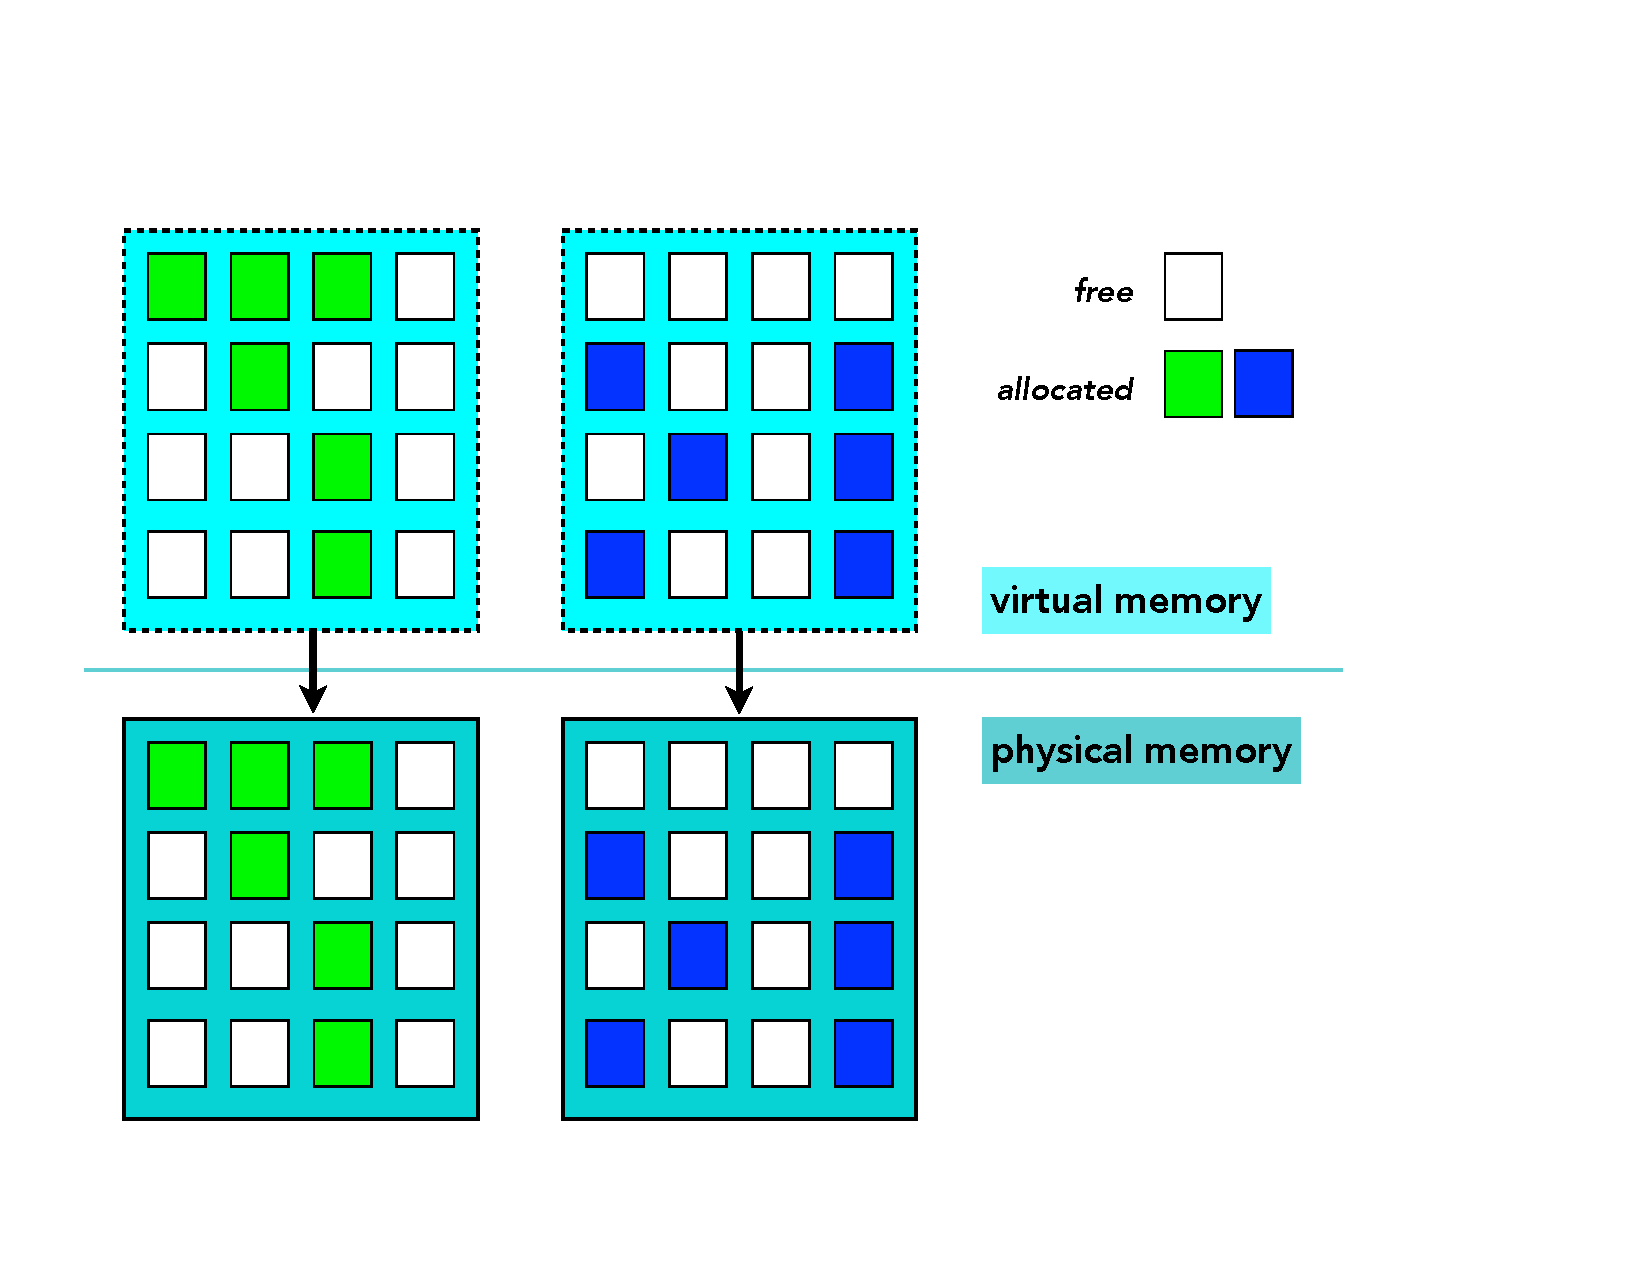
\includegraphics[width=0.45\textwidth]{Chapters/mesh/figures/mesh-diagram-1}
      \label{pre-meshing}
  }
  ~~~~~
  \centering
  \subfloat[\textbf{After:} both virtual pages now point to the
      first physical page; the second page is now freed.]{
      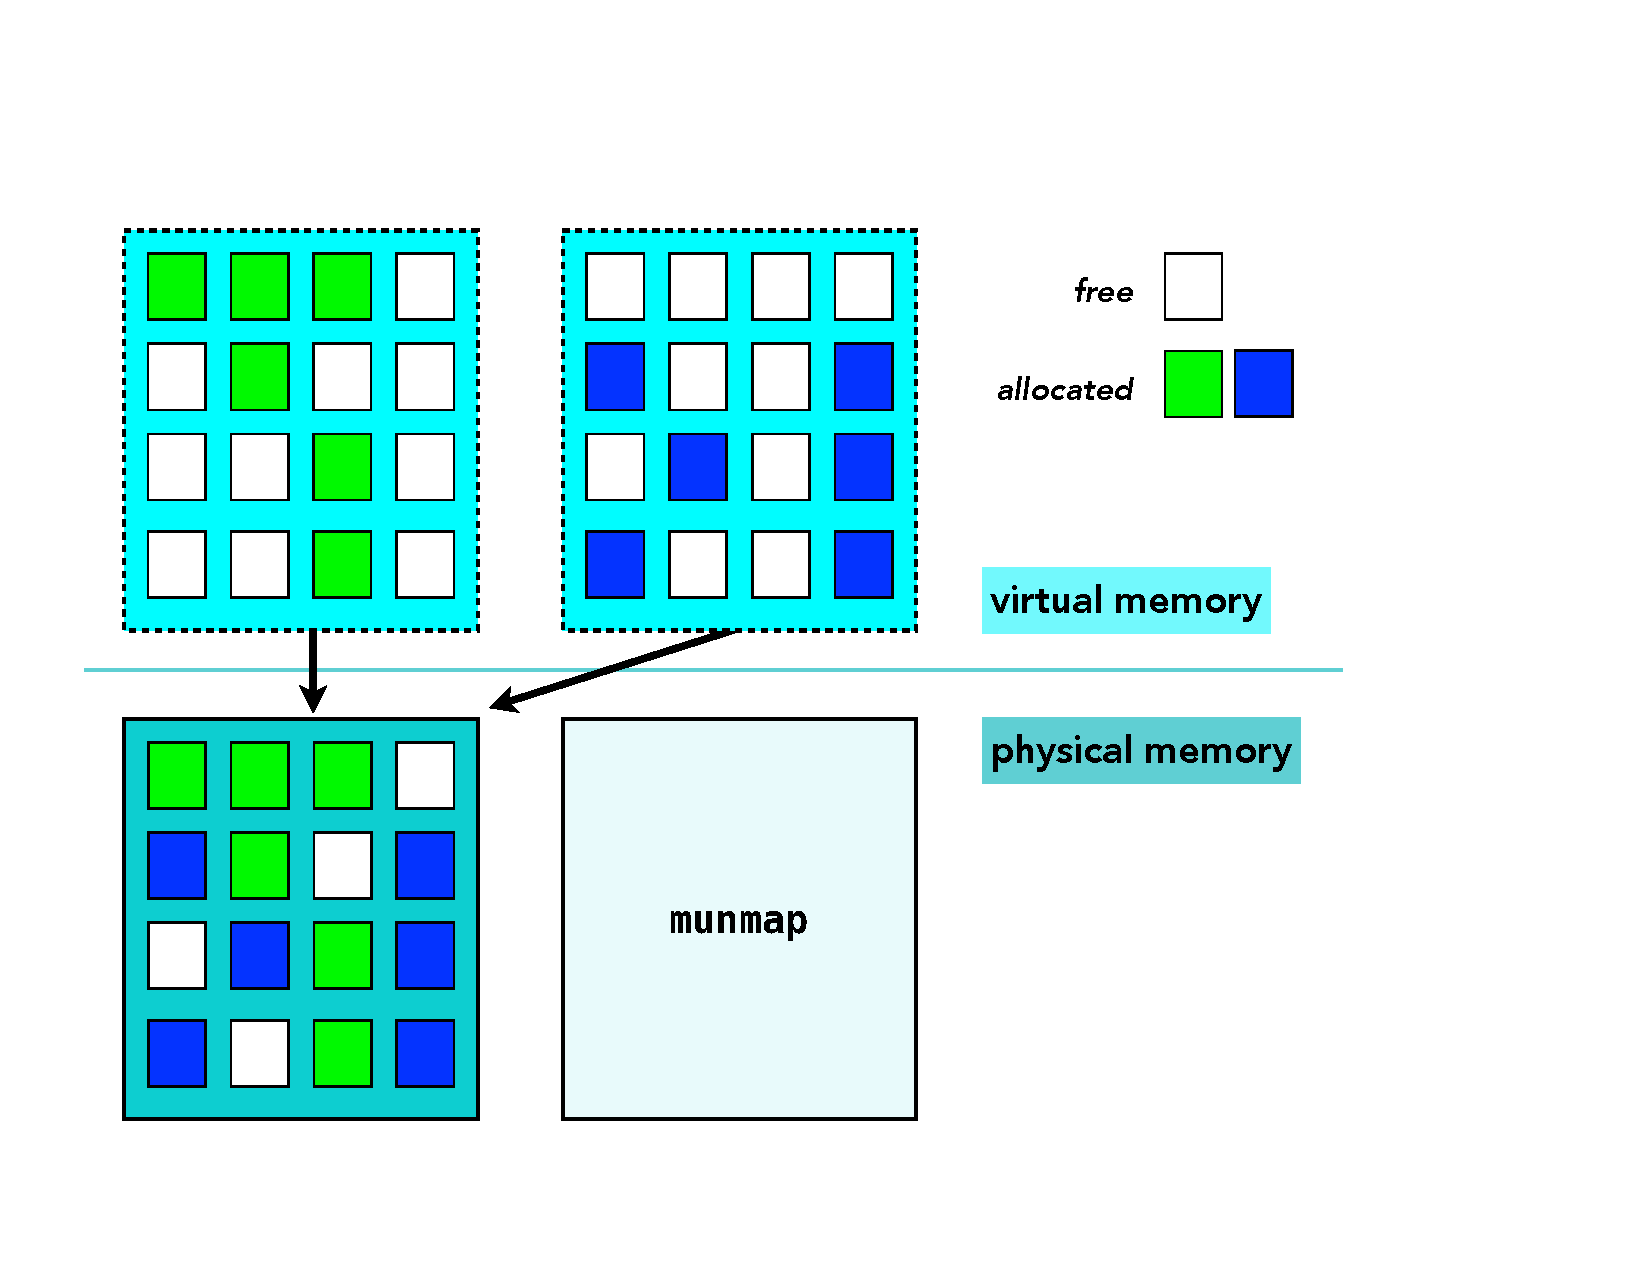
\includegraphics[width=0.45\textwidth]{Chapters/mesh/figures/mesh-diagram-2}
      \label{post-meshing}
  }

  \caption{\textbf{\Mesh{} in action.} \Mesh{} employs novel
    randomized algorithms that let it efficiently find and then
    ``mesh'' candidate pages within \emph{spans} (contiguous 4K pages)
    whose contents do not overlap.  In this example, it increases
    memory utilization across these pages from 37.5\% to 75\%, and
    returns one physical page to the OS (via \texttt{munmap}),
    reducing the overall memory footprint. \Mesh{}'s randomized
    allocation algorithm ensures meshing's effectiveness with high
    probability.}

  \label{fig:meshing}
\end{figure*}


\iffalse
\begin{figure*}[t!]
  \centering
  {
      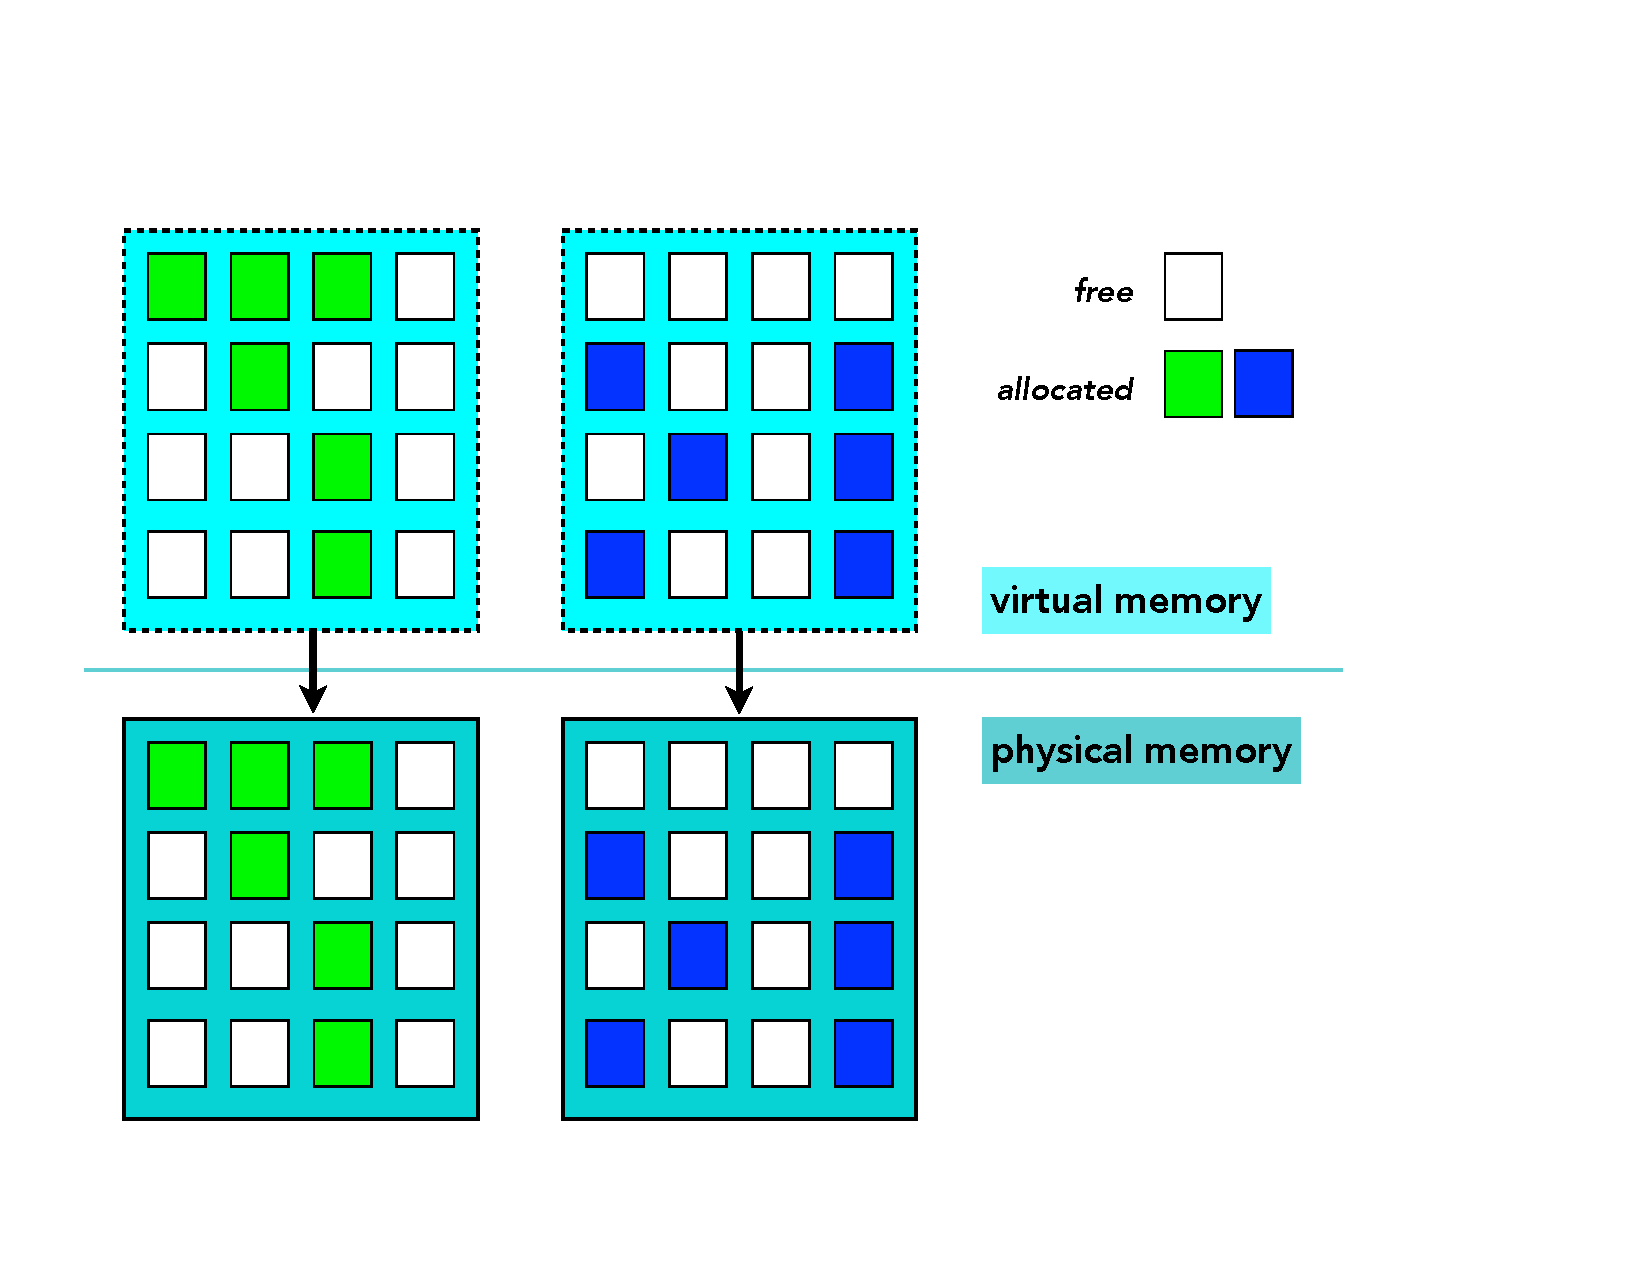
\includegraphics[width=0.45\textwidth]{Chapters/mesh/figures/mesh-diagram-1}
  }

  \caption{\textbf{\Mesh{} in action.} \Mesh{} employs novel
    randomized algorithms that let it efficiently find and then
    ``mesh'' candidate pages within \emph{spans} (contiguous 4K pages)
    whose contents do not overlap.  In this example, it increases
    memory utilization across these pages from 37.5\% to 75\%, and
    returns one physical page to the OS (via \texttt{munmap}),
    reducing the overall memory footprint. \Mesh{}'s randomized
    allocation algorithm ensures meshing's effectiveness with high
    probability.}

  \label{fig:meshing}
\end{figure*}
\fi

\section{Introduction}
\label{sec:introduction}

Memory consumption is a serious concern across the spectrum of modern
computing platforms, from mobile to desktop to datacenters. For
example, on low-end Android devices, Google reports that more than 99
percent of Chrome crashes are due to running out of memory when
attempting to display a web page~\cite{hara:stateofblink}. On
desktops, the Firefox web browser has been the subject of a five-year
effort to reduce its memory footprint~\cite{awsy}. In datacenters,
developers implement a range of techniques from custom allocators to
other \emph{ad hoc} approaches in an effort to increase memory
utilization~\cite{jemalloc:exposehints,redis:announcement}.
%% while
%% Google reports that 10\% of CPU cycles in their clusters are spent on
%% memory allocation~\cite{kanev:2015:warehouse-scale}.

A key challenge is that, unlike in garbage-collected environments,
automatically reducing a C/C++ application's memory footprint
via compaction is not possible. Because the addresses of allocated
objects are directly exposed to programmers, C/C++ applications can
freely modify or hide addresses.  For example, a program may stash
addresses in integers, store flags in the low bits of aligned
addresses, perform arithmetic on addresses and later reference them,
or even store addresses to disk and later reload them.  This hostile
environment makes it impossible to safely relocate objects: if an
object is relocated, all pointers to its original location must be
updated. However, there is no way to safely update \emph{every}
reference when they are ambiguous, much less when they are absent.

Existing memory allocators for C/C++ employ a variety of
best-effort heuristics aimed at reducing average
fragmentation~\cite{johnstone:1998:fragmentation}. However, these
approaches are inherently limited. In a classic result, Robson showed
that all such allocators can suffer from catastrophic
memory fragmentation~\cite{robson:1977:worstcasefrag}. This increase
in memory consumption can be as high as the $\log$ of the ratio
between the largest and smallest object sizes allocated. For example,
for an application that allocates 16-byte and 128KB objects, it is
possible for it to consume $13\times$ more memory than required.

%Embedded systems designed for the Internet-of-Things (IoT), such as the Raspberry Pi Zero W, ship with wireless networking, 3D graphics, and complete operating system stacks but only hundreds of megabytes of memory~\cite{rpi:zero}, placing memory at a premium.

%% TODO: talk about / cite Detlefs paper on precise GC for C/C++

%% address manipulations.  XOR encoding of linked lists

% These addresses can then be freely manipulated: it is legal for C and C++ programs to

% Here, we define fragmentation as the
%amount of memory actually consumed divided by the amount of memory
%actually needed (the total live size).

\begin{comment}
  The result is that C and C++ programs can suffer from fragmentation
(both internal and external). In a setting where compaction
is possible, fragmentation can always be eliminated by squeezing out
space between objects. Since relocating objects is impossible,
fragmentation in C and C++ can become problematic.
\end{comment}

\begin{comment}
  % Push to related work
In languages like LISP, Java and
~\cite{hansen:1969:compaction,fenichel:1969:compaction}, the runtime
system can, as part of garbage collection, periodically compact memory
by moving live objects together. Compaction reduces the working set of
an application and can ensure that an application's footprint never
exceeds some pre-established maximum. Contemporary runtimes like the
Hotspot JVM~\cite{microystems2006memory}, the .NET
VM~\cite{microsoft:dotnet-gc}, and the SpiderMonkey JavaScript
VM~\cite{mozilla:spidermonkey-compaction} implement compaction as part
of their garbage collection algorithms.
\end{comment}


% additionally: build invalid addresses but never dereference them

% emacs pickle state?

%For example, on modern
%systems with a 4 KiB page size and a 16-byte minimum object size, this
%factor corresponds to a worst-case fragmentation of approximately
%$7\times$. In practice, of course, fragmentation is rarely so extreme,
%b
%% TODO: Memory remains one of the scarcest resources across the spectrum of modern computing devices, ranging from servers to desktops to mobile platforms.

%% Not sure - For example, Google reports that \emph{99 percent} of Chrome crashes on low-end Android devices are caused by it running out of memory when attempting to display the page~\cite{hara:stateofblink}.

%% TODO: cost of memory on Amazon servers!

Despite nearly fifty years of conventional wisdom indicating that
compaction is impossible in unmanaged languages, this paper shows that
it is not only possible but also practical. It introduces
\Mesh, a memory allocator that effectively and efficiently performs
compacting memory management to reduce memory usage in unmodified
C and C++ applications.

Crucially and counterintuitively, \Mesh performs compaction without
relocation; that is, without changing the addresses of objects. This
property is vital for compatibility with arbitrary C/C++
applications. To achieve this, \Mesh{} builds on a mechanism which we
call \emph{meshing}, first introduced by Novark et al.'s Hound memory
leak detector~\cite{1542521}. Hound employed meshing in an effort to avoid
catastrophic memory consumption induced by its memory-inefficient
allocation scheme, which can only reclaim memory when every object on
a page is freed. Hound first searches for pages whose live objects do
not overlap. It then copies the contents of one page onto the other,
remaps one of the \emph{virtual} pages to point to the single
\emph{physical} page now holding the contents of both pages, and
finally relinquishes the other physical page to the
OS. Figure~\ref{fig:meshing} illustrates meshing in action.

\Mesh{} overcomes two key technical challenges of meshing that previously made
it both inefficient and potentially entirely ineffective. First,
Hound's search for pages to mesh involves a linear scan of pages on
calls to \texttt{free}. While this search is more efficient than a
naive $O(n^2)$ search of all possible pairs of pages, it remains
prohibitively expensive for use in the context of a general-purpose
allocator. Second, Hound offers no guarantees that \emph{any} pages
would ever be meshable.  Consider an application that happens to
allocate even one object in the same offset in every page. That layout
would preclude meshing altogether, eliminating the possibility of
saving any space.

\Mesh makes meshing both efficient and provably effective (with high
probability) by combining it with two novel randomized
algorithms. First, \Mesh uses a space-efficient randomized
allocation strategy that effectively scatters objects within each
virtual page, making the above scenario provably exceedingly
unlikely. Second, \Mesh incorporates an efficient randomized
algorithm that is guaranteed with high probability to quickly find
candidate pages that are likely to mesh. These two algorithms work in
concert to enable formal guarantees on \Mesh's effectiveness. Our
analysis shows that \Mesh breaks the above-mentioned Robson worst
case bounds for fragmentation with high
probability~\cite{robson:1977:worstcasefrag}, as memory reclaimed by meshing is available for use by any size class.
This ability to redistribute memory from one size class to another enables Mesh to adapt to changes in an application's allocation behavior in a way other segregated-fit allocators cannot.


We implement \Mesh as a library for C/C++ applications running on
Linux or Mac OS X. \Mesh{} interposes on memory management operations,
making it possible to use it without code changes or
recompilation by setting the appropriate environment variable to load
the \Mesh{} library (e.g., \texttt{export
  LD\_PRELOAD=libmesh.so} on Linux). Our evaluation demonstrates that
our implementation of \Mesh{} is both fast and efficient in
practice. It generally matches the performance of state-of-the-art
allocators while guaranteeing the absence of catastrophic
fragmentation with high probability. In addition, it occasionally
yields substantial space savings: replacing the standard allocator
with \Mesh{} automatically reduces memory consumption by 16\%
(Firefox) to 39\% (Redis).
%In
%general, the longer-lived and more memory-intensive the application,
%the more memory \Mesh can save.


\subsection{Contributions}
\label{sec:contributions}

This paper makes the following contributions:

\begin{itemize}

\item It introduces \textbf{\Mesh}, a novel memory allocator that acts
  as a plug-in replacement for \texttt{malloc}. \Mesh{} combines
  remapping of virtual to physical pages (meshing) with randomized
  allocation and search algorithms to enable safe and effective
  \emph{compaction without relocation} for C/C++
  (\S\ref{sec:meshing}, \S\ref{sec:algorithms},
  \S\ref{sec:allocator}).

\item It presents theoretical results that guarantee \Mesh{}'s
    efficiency and effectiveness with high probability (\S\ref{sec:theory}).

\item It evaluates \Mesh{}'s performance empirically, demonstrating \Mesh{}'s ability to reduce
    space consumption while generally imposing low runtime
    overhead (\S\ref{sec:evaluation}).

\end{itemize}
